\section{Prediction System}
\label{sec:predict}

\looseness -1 We now present intermediate results that guided the design decisions for our prediction system. We did not measure performance on the held-out test set throughout development, making decisions solely based on our validation set. \emph{We did not any find any notable difference between training in temporal order (sorted by resolution date), compared to training in a randomly shuffled order}. Below we present results which show the benefits of our reward design for RL training and retrieval system.  \vspace{0.15cm}

\textbf{Reward Design.} For training with RL, we compare three reward functions:
\begin{enumerate}
  \item \textbf{Only Accuracy} \textit{(Baseline):} \( R = \mathds{1}_{y \equiv y^*} \). Vanilla success rewards are commonly used in literature on LLM RL with verifiable rewards~\citep{guo2025deepseek}.
  \item \textbf{Only Brier score} \textit{(\citet{damani2025beyond}):} \( R = S'(q, y, y^*) = -q^2 + \mathds{1}_{y \equiv y^*}\cdot 2q \). This incentivizes both correct predictions and calibrated confidence estimates.
  % Their training reward for calibration in free-form response solely uses our Brier score:\quad \( R = S'(q, y, y^*) = -q^2 + \mathds{1}_{y \equiv y^*}\cdot 2q \). From \Cref{eq:rlcr}, this incentivizes both correct predictions and calibrated confidence estimates.
  \item \textbf{Accuracy + Brier score} \textit{(Ours):} \( R = \mathds{1}_{y \equiv y^*} + S'(q, y, y^*) \). We hypothesise that optimizing the Brier score alone might hurt exploration as when the model assigns a low confidence to its prediction, the correctness has a small impact on the Brier score. To fix this, we propose adding the accuracy term as well. In this case, even on hard questions, which merit low confidence, models get a large boost for correct predictions.
  % that it can be hard for the models to make progress on exploring the outcome space when optimizing the brier score alone. 
\end{enumerate}

\begin{figure}[t]

    \centering
    
    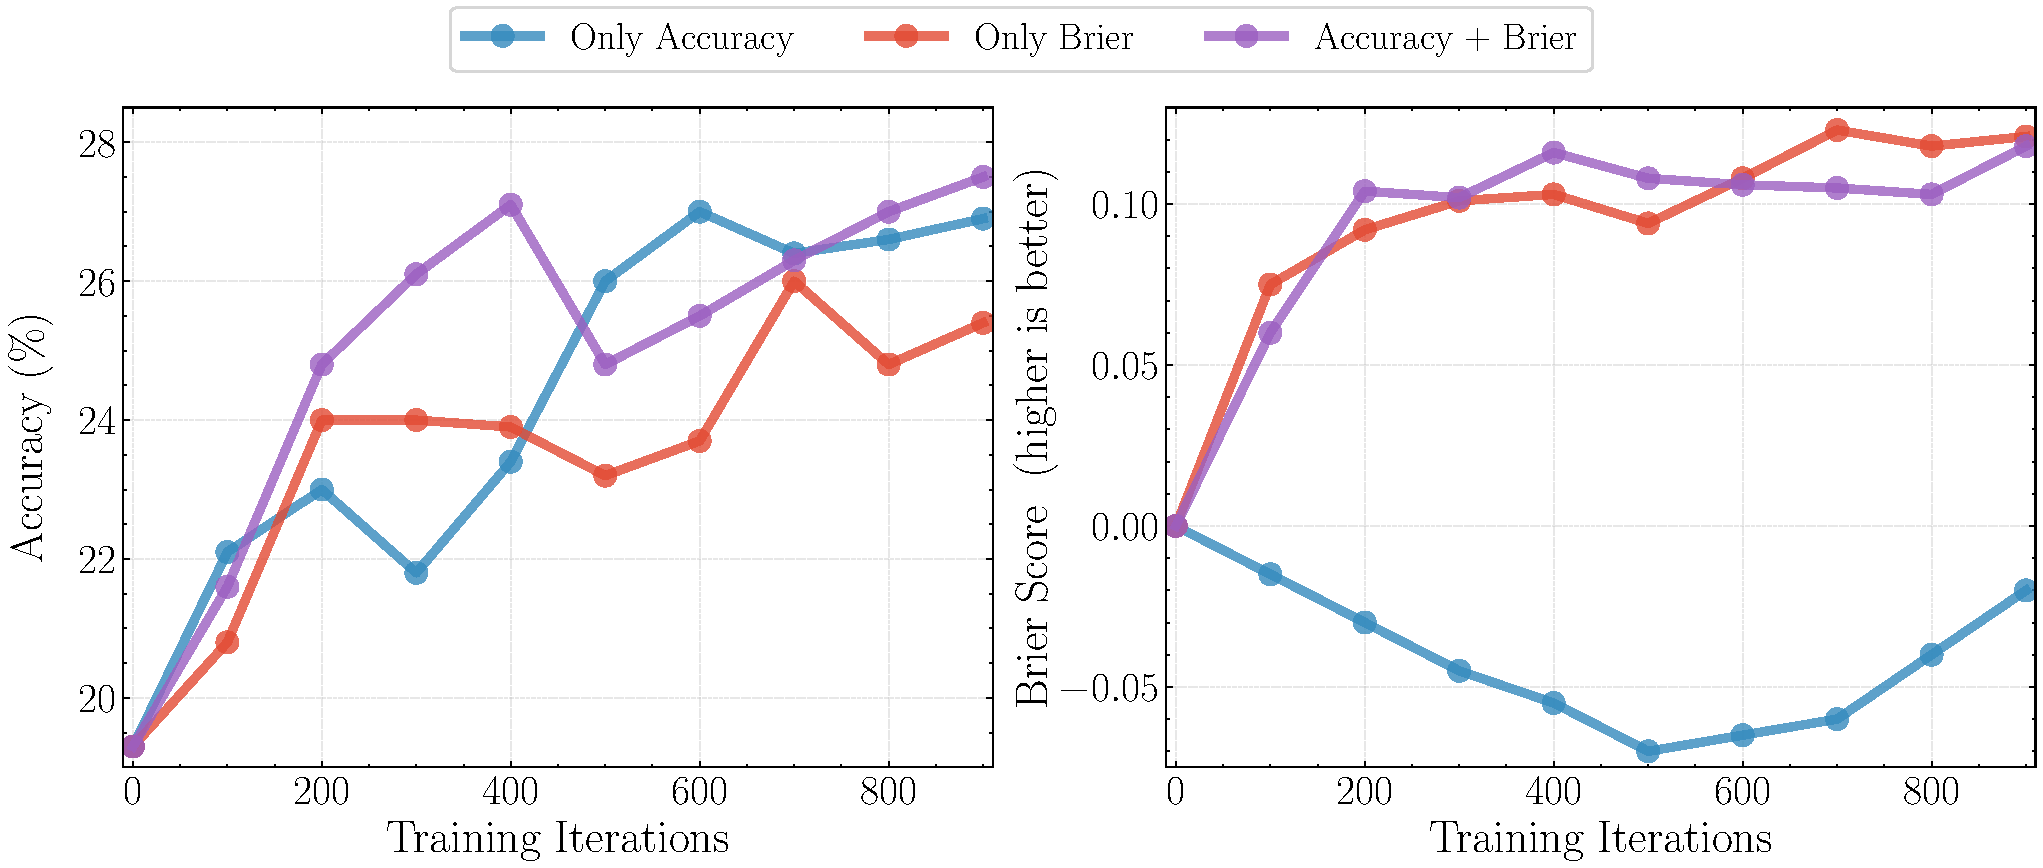
\includegraphics[width=0.99\textwidth]{figures/reward_ablations/training_objectives_recreated.pdf}
     \vspace{-0.25cm} 
    \caption{\textbf{Accuracy + Brier score reward performs the best.} Accuracy alone leads to poor calibration. While brier score incentivizes both correct predictions and calibration, on hard questions with low confidence, it provides little signal on correctness. Adding the accuracy term boosts exploration in this situation.}
    \label{fig:reward_ablations}
    \vspace{-.5cm} 
\end{figure}
\looseness -1 \contribution{Result 3: Accuracy + Brier score as the reward improves performance.} \Cref{fig:reward_ablations} shows the validation set results of training with all three reward functions on the full \ourdataset \ dataset. We observe that optimizing accuracy alone (blue line) leads to negative brier scores, worse than a constant (0) baseline. In contrast, optimizing the Brier score alone (red line) also improves the accuracy, but to a lesser extent. Our proposed reward, accuracy + Brier (purple line), leads to the best performance on both metrics. It improves accuracy beyond the Brier alone while maintaining equal brier score on the validation set. Analyzing output distributions, we find that the brier-only trained model predicts ``Unknown'' with near-0 confidence in $\sim 40\%$ of samples, due to low reward for correct yet low-confidence guesses, which hurts exploration. In contrast, our proposed reward yields ``Unknown'' in only $\sim 4\%$ of samples, making low-confidence guesses on hard cases---improving both accuracy and Brier score. \vspace{0.15cm}

\looseness -1 \textbf{Retrieval.} Like prior work~\citep{zou2022forecasting, halawi2024approaching}, we provide the same relevant recent information across forecasting models. This provides them new evidence, or competing viewpoints to weigh, that was available before the resolution date, but potentially after the model's training cutoff. To prevent leakage issues~\citep{paleka2025pitfalls}, we use our offline CCNews corpus, and only use articles up to \emph{one month} before the question's resolution date. Our overall pool consists of 1 million articles across 60 different sources. We de-duplicate the articles and split each into fixed-size chunks (512 tokens) and embed each chunk with the Qwen3-embedding 8B model. During evaluation, we retrieve the top-$k$ most relevant chunks and append them to the model prompt in order as context. \vspace{0.15cm}

\looseness -1 \textbf{Retrieval leads to large improvements in accuracy.} As shown in \Cref{fig:theguardian_retrieval_acc}, providing retrieved information improves accuracy by $9-18\%$ across model families and sizes. In Appendix~\Cref{fig:articles_retrived}, we vary the number of retrieved chunks and find that improvements plateau after five chunks. Thus, we fix $k=5$ chunks for all evaluations henceforth. % We additionally evaluate \texttt{grok-4.1-fast} with web search tool access and it achieves $90\%$ accuracy on our validation set providing external evidence to the high validity of our question generation recipe. 

\begin{figure}[t]
    \centering
    \vspace{-0.25cm}
        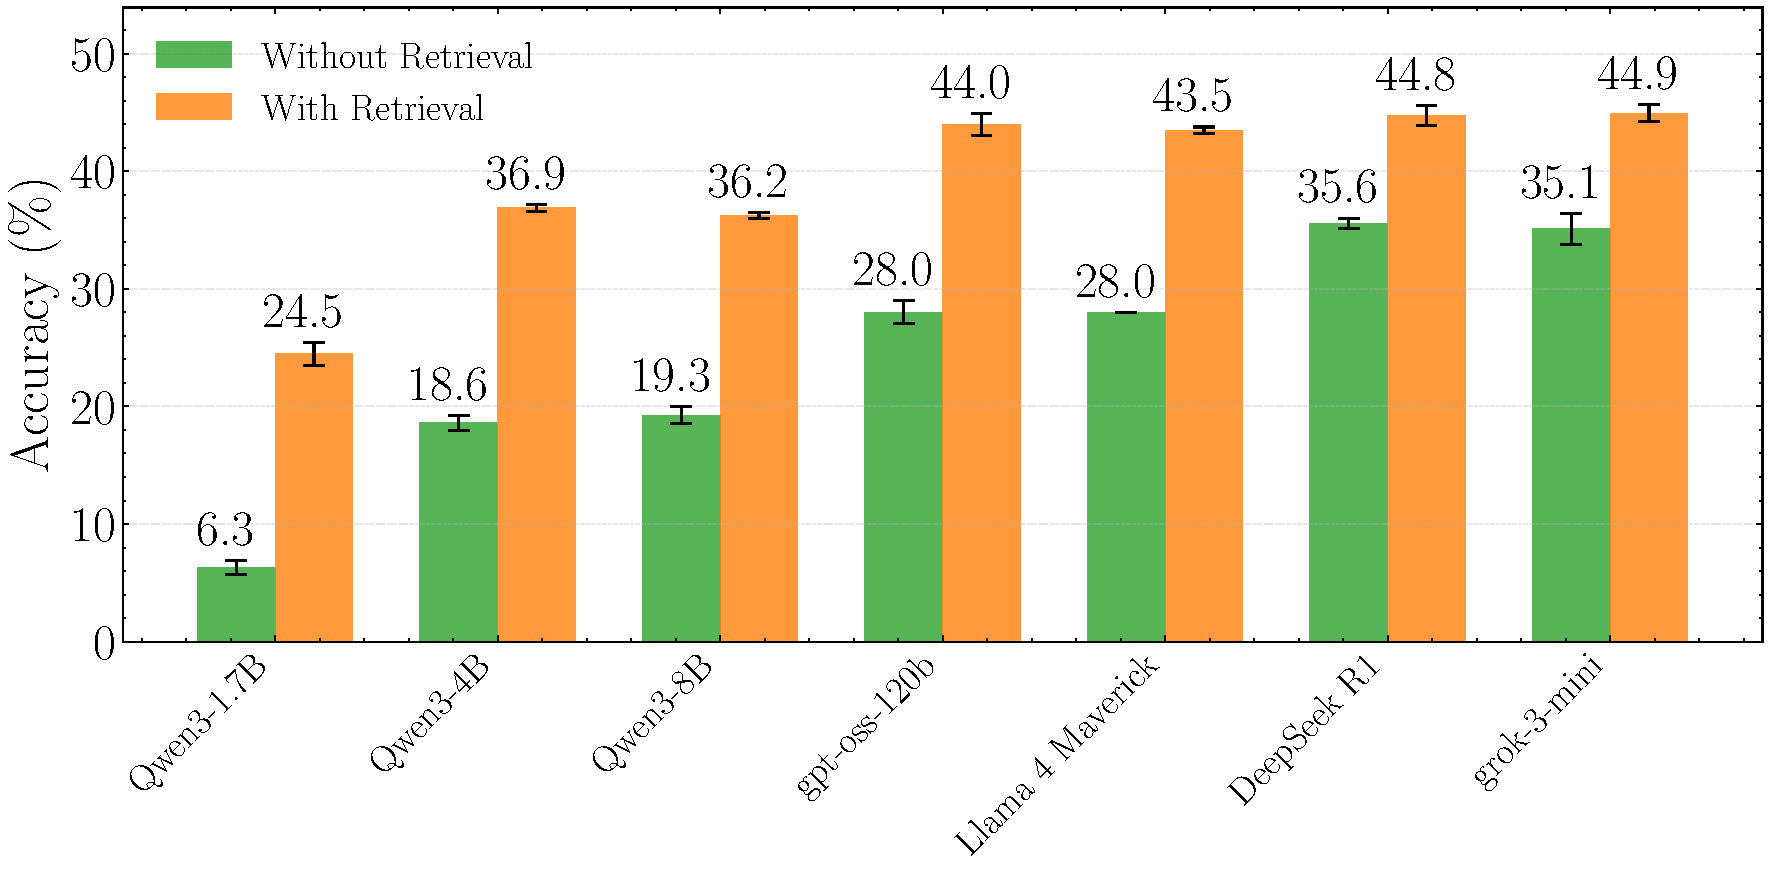
\includegraphics[width=0.8\linewidth]{figures/retrieval/accuracy_comparison_theguardian_207_vs_forcomparison_Llama_4_Scout.pdf}
       
        \label{fig:theguardian_retrieval_acc}
        \vspace{-.35cm} % latex is overrating the gap
    
     \caption{\textbf{Retrieval improves accuracy across models.} We use the specialized Qwen3 8B embedding model to retrieve the 5 most relevant chunks (512 tokens) for each question. We take a cautious approach, using articles only until a month before the resolution date.}
     \vspace{-0.25cm}
\end{figure}

\textbf{Training the final forecasting system.} Based on the above design decisions guided by validation set performance, we now describe our final training methodology: We use the Qwen3-8B embedding model to retrieve the 5 most relevant chunks from news articles until a month before each question's resolution date. During training, we add a random number of such article chunks (between 0 to 5) in the prompt to make our forecaster generalizable to variable number of articles. We train the Qwen3-8B thinking model with GRPO on \ourdataset \ which has $\sim$ 50,000 samples and also include 2000 binary resolved questions from Metaculus (from 2024), both with retrieval. For the reward, we use our Accuracy + Brier score for free-form questions and only brier score for binary questions. We provide configuration details for training and evaluation in \Cref{sec:setupdetails}. %We use Qwen3-4B model (non-thinking) during training for evaluating the accuracy of the responses.


% \vspace{-.2cm} 